
Poly ethyleneglycol (PEG) polymer is made by multiple ethyleneglycol monomers.
Each monomer for building PEG in this tutorial was chosen to be the oxygen atom plus its two neighbor atoms in accordance to the GROMOS united atoms FF (Figure \ref{fig:PEGBBs}).

\begin{figure}
    \centering
    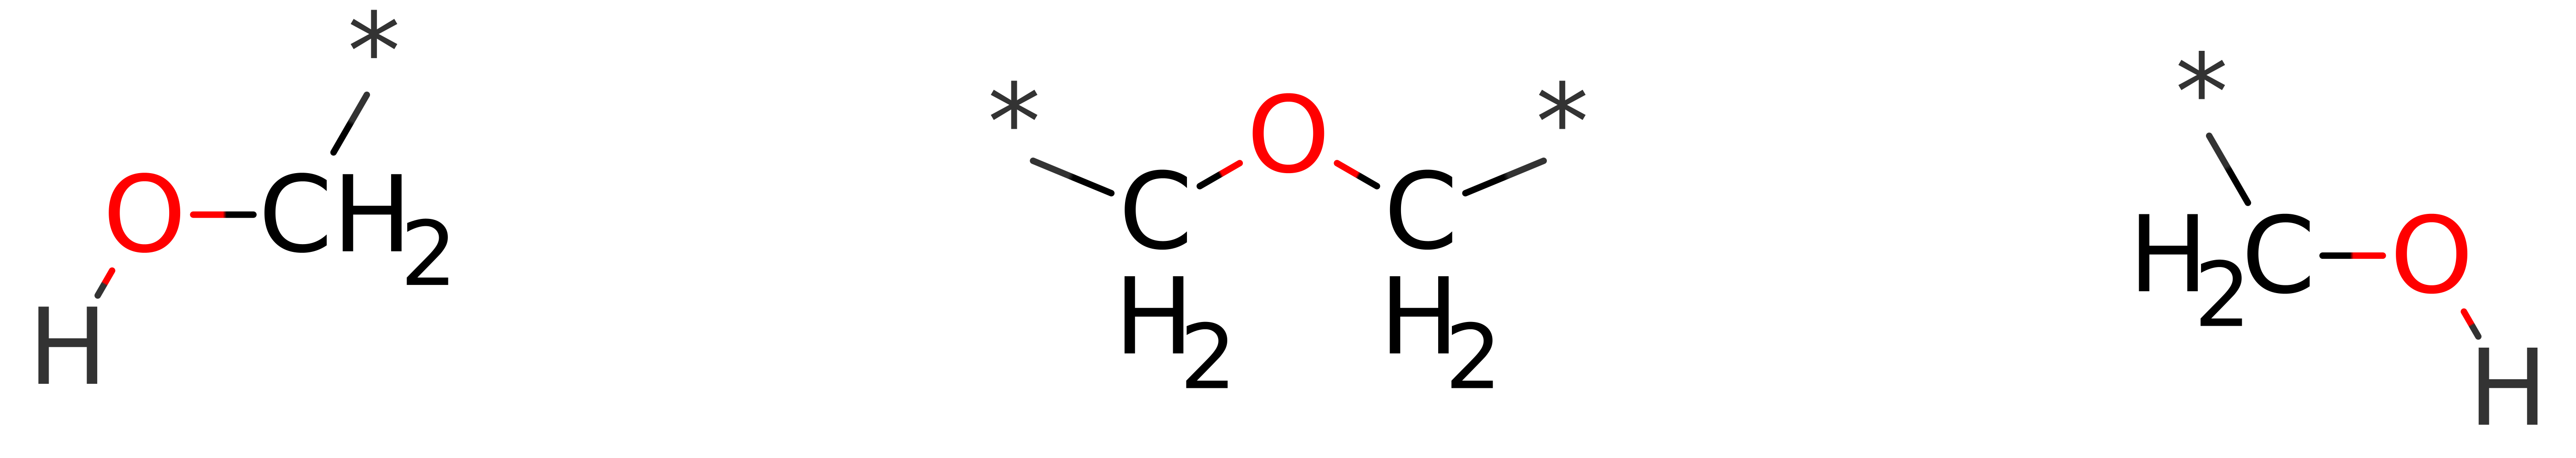
\includegraphics[width=\textwidth]{PEG/PEGBBs.png}
    \caption{PEG BBs. The left and the right monomers are the initial and final monomers, respectively.
            The middle one is the repeating monomer unit.}
    \label{fig:PEGBBs}
\end{figure}

The monomers are pretty simple to be build due to the small number of atoms that need to be defined.
The building blocks as defined in Figure \ref{fig:PEGBBs} are available in the tutorial directory as bb\_PNIP-start.itp, bb\_PNIP.itp and bb\_PNIP-end.itp.

All needed files are provided in the demo directory in pyPolyBuilder root.
\begin{lstlisting}
<path/to/pypolybuilder>/demo/gromacs_format/polymer/PolyEthylene_glycol
\end{lstlisting}
\dirtree{%
.1 PEG.
.2 polyeyhylene-start.itp.
.2 polyeyhylene.itp.
.2 polyeyhylene-end.itp.
.2 list\_param.itp.
.2 connect.in.
.2 connect-4.in.
.2 run.
.3 PEG.sh.
.3 PEG.top.
.3 mdp.
}

The command for building a PEG polymer with 5 monomers is automated in a bash file within tutorial directory called \texttt{how\_to\_run\_this\_example.txt}.
% \begin{figure}
%     \center
%     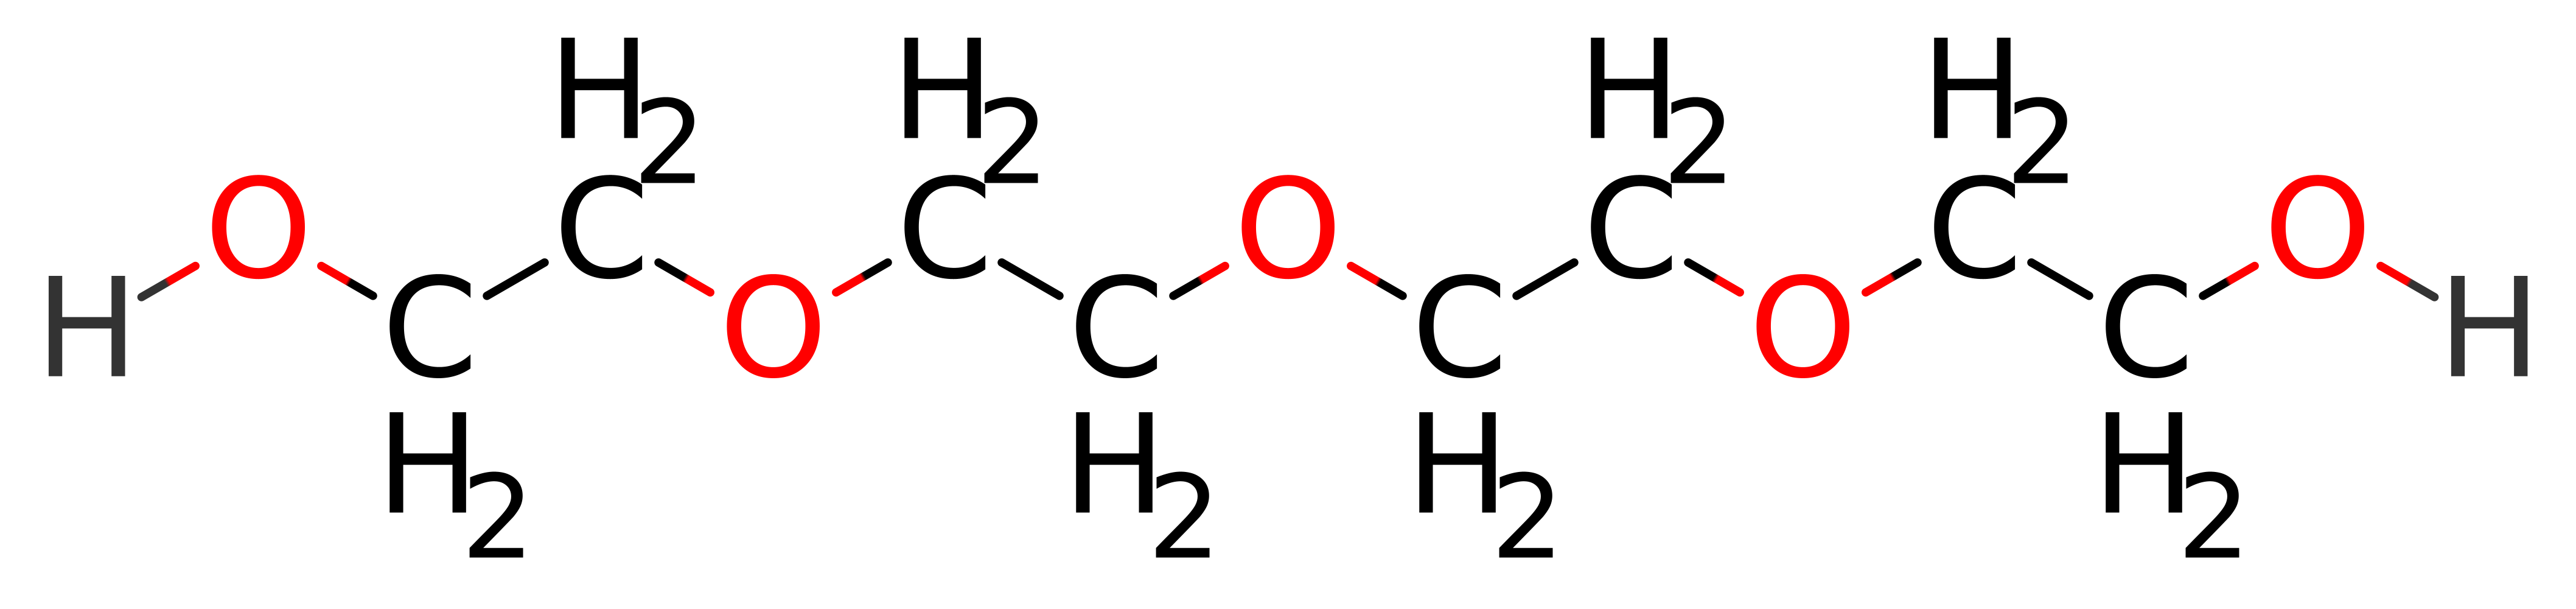
\includegraphics[width=0.5\textwidth]{PEG/PEG.png}
%     \caption{The PEG polymer in the way it is built in this tutorial.}
%     \label{fig:PEG}
% \end{figure}

In order to have a PEG polymer with 5 monomers, with the files provided in the tutorial directory one can use the following command line:

\begin{lstlisting}
python3 ../../../../__main__.py --bbs=etyleneglycol-start.itp,etyleneglycol.itp,etyleneglycol-end.itp --in=connect.in --params=list_param.itp --name=PEG --output=PEG5x.itp --gro=PEG5x.gro --polymer
\end{lstlisting}

Here, \texttt{--bb} option receives the three used BBs: the beginning of the polymer, than the repetition monomer and a final BB.
The connectivity file (named "connect.in") is input through \texttt{--in} option.
FF parameters are defined in \texttt{list\_param.itp} used in \texttt{--params}.
Also, the output is named according to \texttt{--name}, \texttt{--output} and \texttt{--gro}.
At this tutorial, the \texttt{--polymer} flag needs to be used so the network module will be called.

After pyPolyBuilder has finished the optimization step, one can check the molecule geometry in vacuum (Figure \ref{fig:PEGPPB}). 
This initial geometry and the MTFs can be tested by running a MD simulation using the created files.
A script automating a workflow to solvate the polymer and  run a small MD simulation is included in the tutorial directory.

\begin{figure}
    \center
    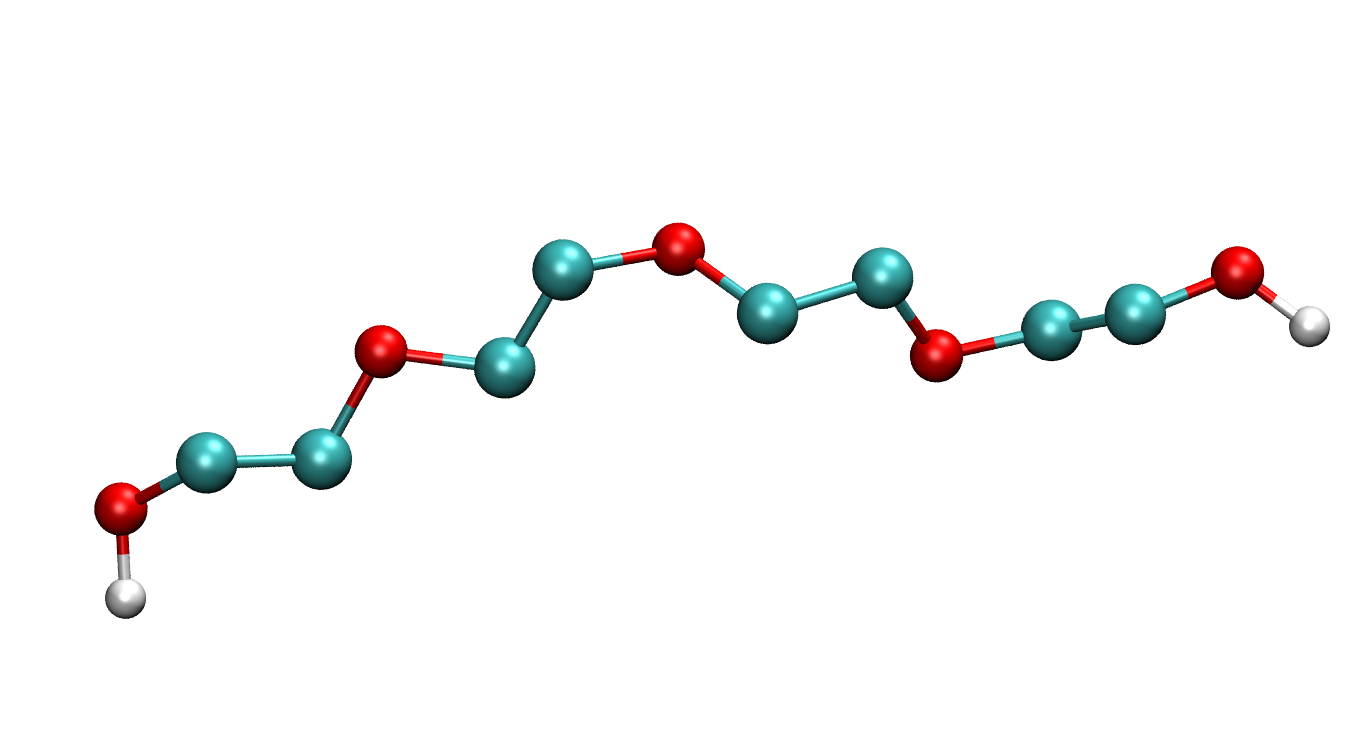
\includegraphics[width=0.5\textwidth]{PEG/PEGPPB.png}
    \caption{The PEG polymer in the way it is built in this tutorial.}
    \label{fig:PEGPPB}
\end{figure}

PEG.sh has the workflow automated but the \texttt{PEG5x.gro} and \texttt{PEG5x.itp} need to be moved to the run directory within tutorial directory and the script needs to be edited in order to use a actual gromacs path on your computer.

Once equilibrated, PEG polymer conformation can be seen as in Figure \ref{fig:PEGSOL}

\begin{figure}
    \center
    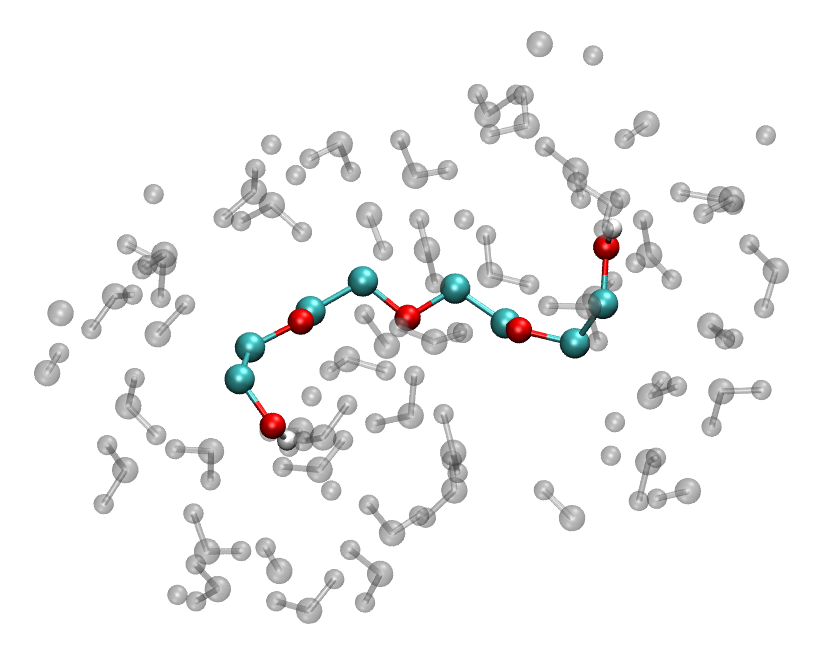
\includegraphics[width=0.5\textwidth]{PEG/PEGSOL.png}
    \caption{The PEG polymer in the way it is built in this tutorial. Water molecules are displayed as translucent silver molecules.}
    \label{fig:PEGSOL}
\end{figure}